\documentclass{beamer}
%\usepackage[latin1]{inputenc}

% Cyrillic support
\usepackage{mathtext}
\usepackage[T2A]{fontenc}
\DeclareSymbolFont{T2Aletters}{T2A}{cmr}{m}{it}
\usepackage[utf8]{inputenc}

% AMS font faces
\usepackage{amsmath, amsfonts, amssymb}

\usepackage{enumerate}

% Tikz package for draw commutative diagrams (include after graphics)
\usepackage{tikz}
\usetikzlibrary{matrix,arrows}
\tikzset{node distance=2cm, auto}

% New commands
\newcommand{\Zfull}{[\mathcal Z^{(1)} + 2\mathcal Z^{(2)}]}
%-------------------------------------------------------------------------------
% New draw commands
\newcommand{\dA}{
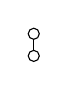
\begin{tikzpicture}
\draw (0pt,2pt) -- (0pt,6pt);
\draw (0pt,0pt) circle (2pt);
\draw (0pt,8pt) circle (2pt);
\end{tikzpicture}
} 

\newcommand{\dB}{
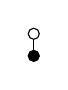
\begin{tikzpicture}
\draw (0pt,2pt) -- (0pt,6pt);
\draw[fill] (0pt,0pt) circle (2pt);
\draw (0pt,8pt) circle (2pt);
\end{tikzpicture}
} 

\newcommand{\dAA}{
\begin{tikzpicture}
\draw (0pt,0pt) -- (0pt,8pt);
\draw (0pt,0pt) -- (8pt,0pt);
\draw (8pt,8pt) -- (0pt,8pt);
\draw (8pt,8pt) -- (8pt,0pt);
\end{tikzpicture}
} 

\newcommand{\dBB}{

\begin{tikzpicture}
\draw[line width=1.5pt] (0pt,0pt) -- (0pt,8pt);
\draw[line width=1.5pt] (0pt,0pt) -- (8pt,0pt);
\draw (8pt,8pt) -- (0pt,8pt);
\draw (8pt,8pt) -- (8pt,0pt);
\end{tikzpicture}
} 

\usetheme{Warsaw}
\title{Гипероктаэдральные комбинаторные типы}
\author{Сергей Воробьев}
\institute{Санкт-Петербургский Государственный университет}
\date{2012}
\begin{document}

\begin{frame}
\titlepage
\begin{center}
\begin{small}
Научный руководитель Константин Игоревич Пименов
\end{small}
\end{center}
\end{frame}


\begin{frame}{Введение}
Комбинаторные типы (species) $F\colon \mathbb{B} \rightarrow
\mathbf{Set}$ (Joyal, 1990-ые). Определил сумму, произведение и композицию
(через композицию аналитических функторов).

Комбинаторная интерпретация --- структуры на точках.
\begin{figure}
   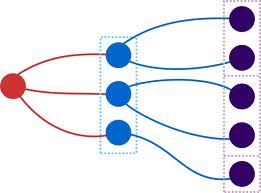
\includegraphics[height=15mm]{species.jpg}
\end{figure}

Гипероктаэдральные комбинаторные типы
(H-species) $F\colon \mathbb{HB} \rightarrow \mathbf{HSet}$ (Bergeron, 1996).
Определил сумму, произведение, но остался вопрос о композиции.

Комбинаторная интерпретация --- структуры на гранях куба?
$$
\dA, \dB, \dAA, \dBB
$$
\end{frame}

\begin{frame}{Постановка задачи}
\begin{enumerate}[*]
\item Разработать комбинаторный язык для h-species.
\item Определить композицию h-species
\end{enumerate}
\end{frame}

\begin{frame}{Аналитический функтор}
Аналитический функтор является левым расширением по Кану функтора $F$
относительно $i$.
\begin{center}
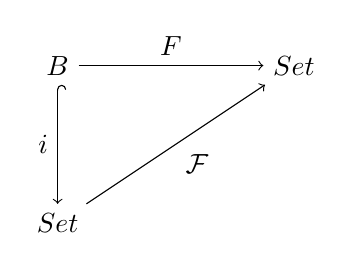
\begin{tikzpicture}
	\node (B) {$B$};
	\node (S1) [below of=B] {$Set$};
	\node (S2) [right of=B, node distance=3cm] {$Set$};
	\draw [right hook->] (B) to node [swap] {$i$} (S1);
	\draw [->] (B) to node {$F$} (S2);
	\draw [->] (S1) to node [swap] {$\mathcal F$} (S2);	
\end{tikzpicture}
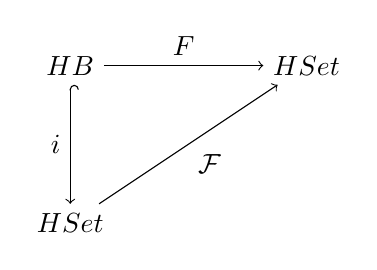
\begin{tikzpicture}
	\node (B) {$HB$};
	\node (S1) [below of=B] {$HSet$};
	\node (S2) [right of=B, node distance=3cm] {$HSet$};
	\draw [right hook->] (B) to node [swap] {$i$} (S1);
	\draw [->] (B) to node {$F$} (S2);
	\draw [->] (S1) to node [swap] {$\mathcal F$} (S2);
\end{tikzpicture}
\end{center}
$$
\mathcal F = \sum\limits_n F[n] \times A^{n} / S_n
$$                   
$$
\mathcal F = \sum\limits_n F[\Bar n] \times A^{\Bar n} / B_n
$$
Где $A^{\Bar n}$ задает отображение, сохраняющее инволюцию. Это раскраска.
\end{frame}

\begin{frame}{Цикленный индекс}
Цикленный индекс --- результат декатегорификации аналитического функтора.
Морфизм из моноидальной категории в какую-либо алгебру. Новое: моноцвета и
бицвета. Моноструктуры и биструктуры. В отличии от обычных species, для
h-species разумно рассматривать пару $(\mathcal Z^{(1)}, \mathcal Z^{(2)})$ ---
для моноструктур и биструктур. Удобно рассмотреть базис $\psi_{x}, \psi_{x, y,
y}$.
\end{frame}

\begin{frame}{Формулы для цикленного индекса}
Species
$$
\mathcal Z_F = 
\sum_{n, \lambda \vdash n}\chi(\sigma_{\lambda})
\frac{\psi_{x}^{\lambda}}{z_{\lambda}}
$$

H-species
\begin{equation}
\label{eq:h-fr2}
\mathcal Z_F^{(1)} = 
\sum_{n, \lambda_o^1 + \lambda_o^2 + \lambda_e^1 + \lambda_e^2 \vdash
n}\chi(\sigma_{\lambda_o^1 \lambda_o^2 \lambda_e^1 \lambda_e^2})
\frac{\psi_{x, y, y}^{\lambda_e^1 + \lambda_o^2} \psi_{x}^{\lambda_e^2 + 
\lambda_o^1}}{z_{\lambda_o^1 \lambda_o^2 \lambda_e^1 \lambda_e^2}}
\end{equation}

\begin{equation}
\begin{split}
\mathcal Z_F^{(2)} = 
\frac{1}{2}&
\sum_{n, \lambda^1 + \lambda^2 \vdash n}\chi(\sigma_{\lambda^1 \lambda^2})
\frac{\psi_{x, y, y}^{\lambda^1} \psi_{x}^{\lambda^2}}{z_{\lambda^1 \lambda^2}}
- \\
\frac{1}{2}&
\sum_{n, \lambda_o^1 + \lambda_o^2 + \lambda_e^1 + \lambda_e^2 \vdash
n}\chi(\sigma_{\lambda_o^1 \lambda_o^2 \lambda_e^1 \lambda_e^2})
\frac{\psi_{x, y, y}^{\lambda_e^1 + \lambda_o^2} \psi_{x}^{\lambda_e^2 + 
\lambda_o^1}}{z_{\lambda_o^1 \lambda_o^2 \lambda_e^1 \lambda_e^2}}
\end{split}
\end{equation}

Где $\lambda_o$ --- циклы нечетной длинны, $\lambda_e$ ---
циклы четной длинны.
\end{frame}

\begin{frame}{Формулы для композиционного произведения}
Species:
\begin{equation*}
\begin{split}
	\mathcal Z_{F \circ G} (\psi_x^1, \psi_x^2, \psi_x^3, \dots ) = \mathcal Z_F(
		&\mathcal Z^{(1)}_G(\psi_x^1, \psi_x^2, \psi_x^3, \dots), 
		\mathcal Z^{(1)}_G(\psi_x^2, \psi_x^4, \psi_x^6, \dots), \\ 
		&\mathcal Z^{(1)}_G(\psi_x^3, \psi_x^6, \psi_x^9, \dots), 
		\dots)
\end{split}
\end{equation*}

H-Species:
\begin{equation*}
\begin{split}
	\mathcal Z^{(1)/(2)}_{F \circ G} (&\psi_x^1, \psi_x^2, \psi_x^3, \dots, 
	\psi_{x,y,y}^1, \psi_{x,y,y}^2, \psi_{x,y,y}^3, \dots) = \\
	\mathcal Z_F^{(1)/(2)}(
		&\mathcal Z^{(1)}_G(\psi_x^1, \psi_x^2, \psi_x^3, \dots, 
					 \psi_{x, y, y}^1, \psi_{x, y, y}^2, \psi_{x, y, y}^3, \dots), \\
		&\mathcal Z^{(1)}_G(\psi_x^2, \psi_x^4, \psi_x^6, \dots, 
					 \psi_{x, y, y}^2, \psi_{x, y, y}^4, \psi_{x, y, y}^6, \dots), \\
		&\mathcal Z^{(1)}_G(\psi_x^3, \psi_x^6, \psi_x^9, \dots, 
					 \psi_{x, y, y}^3, \psi_{x, y, y}^6, \psi_{x, y, y}^9, \dots), \dots, \\
		&\Zfull_G(\psi_x^1, \psi_x^2, \psi_x^3, \dots, 
					 \psi_{x,y,y}^1, \psi_{x,y,y}^2, \psi_{x,y,y}^3, \dots), \\
		&\Zfull_G(\psi_x^2, \psi_x^4, \psi_x^6, \dots, 
					 \psi_{x,y,y}^2, \psi_{x,y,y}^4, \psi_{x,y,y}^6, \dots), \\
		&\Zfull_G(\psi_x^3, \psi_x^6, \psi_x^9, \dots, 
					 \psi_{x,y,y}^3, \psi_{x,y,y}^6, \psi_{x,y,y}^9, \dots), \dots
	)
\end{split}	
\end{equation*}
\end{frame}

\begin{frame}{Примеры}
\begin{enumerate}[(1)]
\item
$$
\Zfull(\dB \times \dB) = \Zfull(\dB) \times \Zfull(\dB) =(\psi_{x, y, y}^1)^2
$$
Произведение сохраняется для $\mathcal Z^{(1)}, \Zfull$.
\item
$$A \circ \dB = \dB \circ A = A$$
\dB --- единица подстановки.
\item
$$\dBB \circ \dA = \dAA$$
Подстановка \dA, это <<стирание различий между противоположными
гранями>>.
\end{enumerate}
\end{frame}

\begin{frame}{Заключение}
Результат:
\begin{enumerate}[*]
\item Частично разработан комбинаторный язык для h-species.
\item Написана явная формула для цикленного индекса.
\item Написана формула для композиции цикленных индексов.
\item Произведены явные вычисления для нескольких содержательных примеров,
результаты согласуются с комбинаторной интуицией и помогают ее развить.
\end{enumerate}
\end{frame}

\end{document}
